\documentclass[t]{beamer}
\setbeamertemplate{navigation symbols}{} %no nav symbols
\usepackage{beamerthemeshadow}
\usepackage{pgf}
\usepackage{listing}
\usepackage{listings}
\usepackage{verbatim}
\usepackage{multirow}
\usetheme{Copenhagen} % Beamer theme v 3.0
\usecolortheme{whale} % Beamer color theme


\usepackage[boxed,linesnumbered,vlined,slide]{algorithm2eCustom}



\title[Fall Presentation 2010\hspace{14em}\insertframenumber/\inserttotalframenumber]{Proactive Caching for Spatial Queries in Mobile Environments \\\&\\ Cache Invalidation and Replacement Strategies for Location-Dependent Data in Mobile Environments}
\author[Jeppe R. Thomsen]{Jeppe R. Thomsen}%\\ \small{jenslyn@cs.aau.dk}}
\institute{Hong Kong Polytechnic University\\ Department of Computing}
\begin{document}
\begin{frame} % Cover slide
\titlepage
\end{frame}
% Instead, you can use \frame{\titlepage}} (Beamer v 2.2 macro)
%
%\section{Introduction} % Bookmark information
%
%\begin{frame}[red]
%\frametitle{Overview}
%\Large
%
%\end{frame}

%\section{Cache Invalidation and Replacement Strategies for Location-...}

\subsection{Introduction}

\begin{frame}
\frametitle{Introduction}

	\begin{center}
	\Large
	Published in IEEE Transactions on Computers\\\vspace{1em}
	by\\\vspace{1em}
	Baihua Zheng, Jianliang Xu, and Kik L. Lee\\\vspace{1em}
	October 2002
	\end{center}

\end{frame}


\begin{frame}
\frametitle{Motivation}
\large
Doing location based queries from a mobile phone, with a cache, the user could:
\begin{itemize}
\item Save Money
\item Reduce Network Traffic
\item Conserve battery
\end{itemize}

\vspace{2em}
Existing cache replacement policies too simple. Does not consider valid scopes of cached items
\vspace{0.5em}

\end{frame}


\begin{frame}
\frametitle{Related Work}

Temporal-dependent invalidation
\begin{itemize}
\item server sends \textit{invalidation reports} to clients
\end{itemize}
\vspace{1em}
Location-dependent invalidation
\begin{itemize}
\item Depending on users location or area after movement, data might be invalidated.
\end{itemize}
\vspace{1em}
Semantic data caching
\begin{itemize}
\item cached items saved with locations associated with query
\end{itemize}

\end{frame}

%----------------------------------------------


\subsection{Problem}

\begin{frame}
\frametitle{Problem}

Mobile, cache enabled, clients communicate with fixed hosts, requesting location based service from fixed hosts. 

A Geometric model is used, with identifying their location via e.g. GPS.

\begin{itemize}
\item Mobile clients
\item Fixed hosts
\item Geometric model
\end{itemize}

\vspace{1em}

- Perceived Problem
\begin{quotation}
	Given a cache enabled client and a LBS server, which cache replacement technique performs best, and does data distribution have an effect.
\end{quotation}
\end{frame}


%----------------------------------------------

\subsection{Contribution}
\begin{frame}
\frametitle{Invalidation Strategies}

Location-Dependent Invalidation Strategies
\hspace{1em}

\begin{itemize}
\item[PE\hspace{0.5em}] Polygonal Endpoints
\item[AC\hspace{0.5em}] Approximate Circle
\item[CEB] Cache Efficientcy Based
\end{itemize}

\hspace{1em}

Methods to support invalidation of cache items based on the valid scope of each items 


\end{frame}


\begin{frame}
\frametitle{CEB - Cache Efficientcy Based}


$E(v^{'}_i)=\frac{A(v^{'}_i)/A(v)}{(D+O(v^{'}_i))/D} = \frac{A(v^{'}_i)D}{A(v)(D+O(v^{'}_i))}$

\begin{itemize}
\item $v^{'}_i$ - subregion of $v$
\item $A(v^{'}_i)$ - area of $v^{'}_i$
\item $O(v^{'}_i)$ - overhead to record scope of $v^{'}_i$
\item $D$ - Data size
\item $A(v^{'}_i)/A(v)$ - Cache hit ratio (assuming uniform probability of queries from all locations)
\item $(D+O(v^{'}_i))/D$ - Cost ratio to archive hit ratio
\item $E(v^{'}_i)$ - Caching efficiency of data item with respect to scope of $v^{'}_i$
\end{itemize}

\end{frame}


\begin{frame}
\frametitle{Cache Replacement Policies}

Eject cache items furthest away from user\\
\vspace{1em}
Favor cache items with larger valid scope\\
\vspace{1em}

\begin{itemize}
\item[PA\hspace{1em}] Probability Area $c_{i,j} = P_i * A(v^{'}_{i,j})$
\item[PAID] Probability Area Inverse Distance  $c_{i,j} = \frac{P_i * A(v^{'}_{i,j})}{D(v^{'}_{i,j})}$
\end{itemize}

\begin{itemize}
\item $c_{i,j}$ - Cost function of data value $j$ of cache item $i$
\item $P_i$ - Access probability of cache item
\item $A(v^{'}_{i,j})$ - Area of attached valid scope $v^{'}_{i,j}$
\item $D(v^{'}_i)$ - Distance between user and valid scope $A(v^{'}_{i,j})$
\end{itemize}

\end{frame}


%----------------------------------------------

\subsection{Experimental Results}

\begin{frame}
\frametitle{Setting}


\begin{columns}
	\begin{column}{0.5\textwidth}
		\only<1>{ 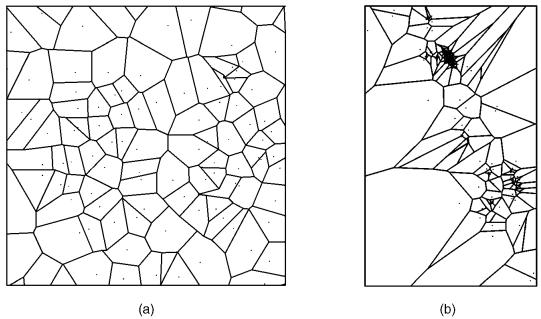
\includegraphics[page=1,scale=0.45]{images/voronoi.jpg}}
	\end{column}
	\begin{column}{0.5\textwidth}
		\begin{itemize}\itemsep 16pt
		\item 2 datasets, modeled as Voronoi Diagrams (110/185 Points)
		\end{itemize}
	\end{column}
\end{columns}
\end{frame}

\begin{frame}

\begin{center}
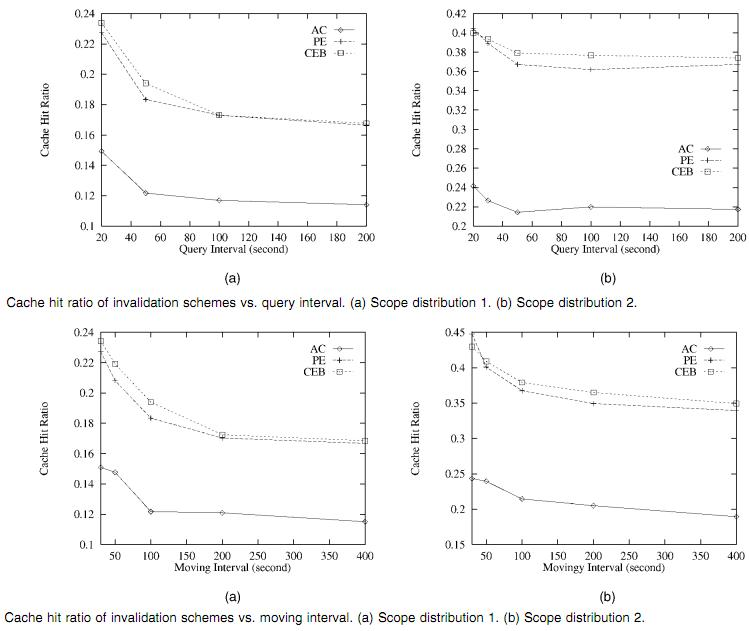
\includegraphics[scale=0.45]{images/fig3-4.jpg}
\end{center}

\end{frame}

\begin{frame}
\frametitle{Cache hit ratio / Data Size - scope 1 and 2}

\begin{center}
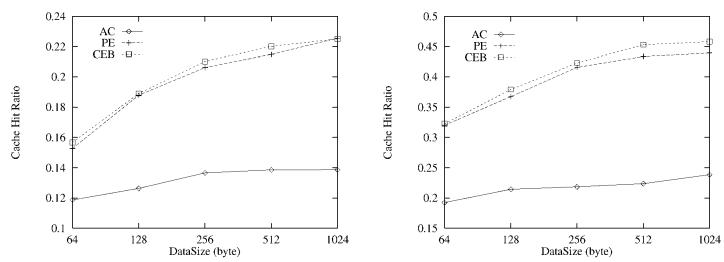
\includegraphics[scale=0.6]{images/fig5.jpg}
\end{center}

\end{frame}

\begin{frame}
\frametitle{Cache hit ratio / Query interval - scope 1 and 2}

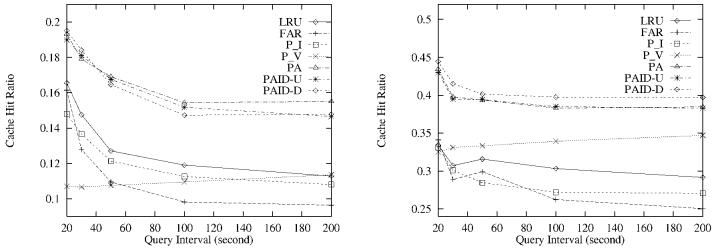
\includegraphics[scale=0.5]{images/fig6.jpg}\\
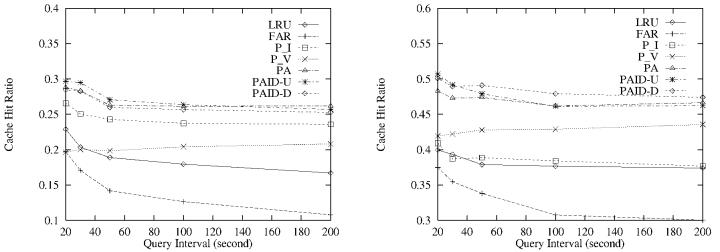
\includegraphics[scale=0.5]{images/fig7.jpg}


\end{frame}

\begin{frame}
\frametitle{Cache hit ratio / Moving interval - scope 1 and 2}

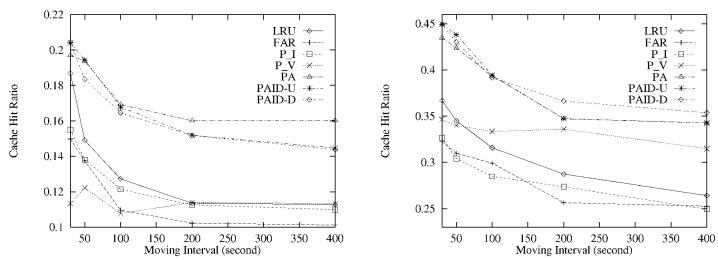
\includegraphics[scale=0.5]{images/fig8.jpg}\\
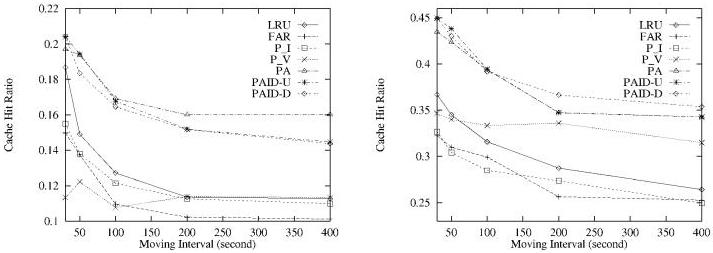
\includegraphics[scale=0.5]{images/fig9.jpg}

\end{frame}


\begin{frame}
\frametitle{Conclusion}
\Large

\textbf{Introduce}
\begin{itemize}
\item CEB
\item PA
\item PAID
\item Data Distance (PAID)
\end{itemize}

Show experimentally that using PA and PAID will give some improvement


\end{frame}

\begin{frame}
\frametitle{Impression}

Paper too long, with very little content\\
\vspace{1em}
Experimental section almost 2/3 of paper.\\
\vspace{1em}
Paper does not state problem to be solved, is a rather just a description of methods\\
\vspace{1em}
Contribution: experimentally showing that obvious improvements to existing ideas works okay.


\end{frame}
%\section{Proactive Caching for Spatial Queries in Mobile Environments}

\subsection{Introduction}

\begin{frame}
\frametitle{Introduction}
	\begin{center}
	\Large
	Published at: ICDE '05: Proceedings of the 21st International Conference on Data Engineering\\\vspace{1em}
	by\\\vspace{1em}
	Haibo Hu, Jianliang Xu, Wing Sing Wong, Baihua Zheng, Dik Lun Lee, and Wang-Chien Lee\\\vspace{1em}
	April 2005
	\end{center}
\end{frame}


\begin{frame}
\frametitle{Motivation}
\large


\end{frame}


\begin{frame}
\frametitle{Related Work}
\Large

Caching:
\begin{itemize}\itemsep 16pt
\item Page Caching
\item Semantic Caching
\end{itemize}

\end{frame}

%----------------------------------------------


\subsection{Problem}

\begin{frame}
\frametitle{Problem}

\end{frame}

\begin{frame}
\frametitle{R-Tree}

\begin{center}
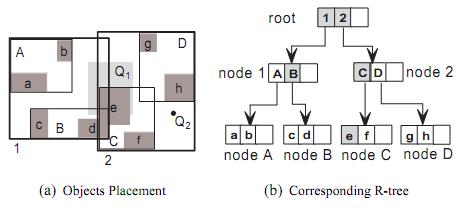
\includegraphics[scale=0.95]{images/r-tree.jpg}
\end{center}
\end{frame}

%----------------------------------------------

\subsection{Contribution}

\begin{frame}
\frametitle{Proactive Caching}

\begin{enumerate}
\item Execute query $Q$ on local partial R-tree index and cache
\item If any items are found while executing $Q$ locally, then return immidiately
\item If $Q$ is satisfied then terminate, else Construct $Q_r = Q + H$ and send to server
\end{enumerate}

\begin{center}
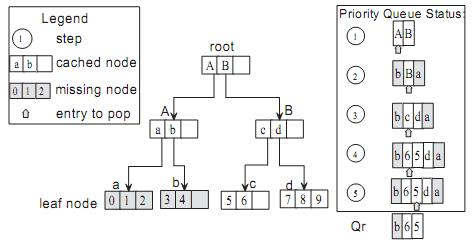
\includegraphics[scale=0.55]{images/kNNproactive-caching.jpg}
\end{center}

\end{frame}

\begin{frame}
\frametitle{Proactive Caching}

\begin{center}
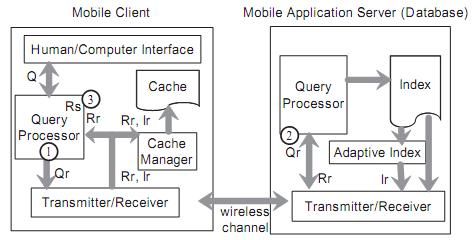
\includegraphics[scale=0.80]{images/proactive-caching.jpg}
\end{center}

\end{frame}

\begin{frame}
\frametitle{Response time and Hit rate}

Query responsetime:\\
$resp(Q)=\frac{|R_r|(T{Q_{r}}+\frac{1}{2}|R_r|\cdot T_d}{|R|}$
\vspace{1.5em}

Cache Hit rate:\\
$hit_c = \frac{|R_s|}{R}$
\end{frame}


\begin{frame}
\frametitle{}

Algorithm is a 2-approximation algorithm

When cached node is removed, the children of that item should be considered into the benifit calculations.

$\sum_{j \in D(i)}{prob(j)\times size(i)+ prob(i)\times size(i)}$


\end{frame}


%----------------------------------------------

\subsection{Experimental Results}
%
%\begin{frame}
%\frametitle{Setting}
%\end{frame}
%
%\begin{frame}
%
%\end{frame}
%
%\begin{frame}
%\frametitle{Cache hit ratio / Data Size - scope 1 and 2}
%
%\end{frame}
%
%\begin{frame}
%\frametitle{Cache hit ratio / Query interval - scope 1 and 2}
%
%\end{frame}
%
%\begin{frame}
%\frametitle{Cache hit ratio / Moving interval - scope 1 and 2}
%%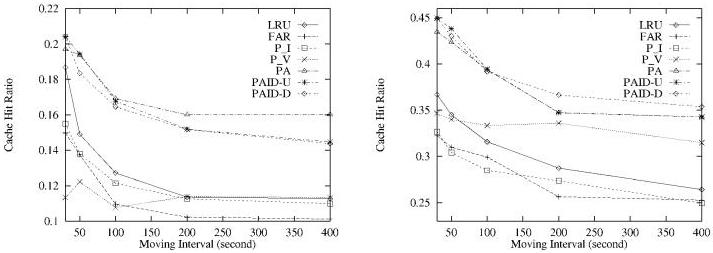
\includegraphics[scale=0.5]{images/fig9.jpg}
%
%\end{frame}
%

\begin{frame}
\frametitle{Conclusion}
\Large
Proactive Caching outperforms page caching and semantic caching
\end{frame}

\begin{frame}
\frametitle{Impression}

Their results were not stellar\\

Graphs are "`cut"' just before compeditors might seem to become better

\end{frame}

\section{Tutorial - Fast Fourier Transformation }

\subsection{Introduction}

\begin{frame}
\frametitle{Related Work}



\end{frame}
%\section{Problem}\label{sec:problem}

In our setting we assume users own an Internet enabled mobile device with positioning capabilities. Users issue \spath queries to an online service provider. Users want the response time, on the return of their \spath result, to be comparable to that of an offline application. We use the terms user query, incoming query, and query interchangeably.

The \spath service provider needs to provide a fast service to its users. The service provider also want to save cost on hardware, such as CPU and HDD space. The \spath provider therefor wants to return as many \spath results as possible, using the least amount of computation and space.

Calculating a \spath will, regardless of the algorithm used, always be an expensive calculation\cite{CNeed}. Using a \spath cache at the \spath service provider can reduce the CPU cycles used in order to return a \spath result. Doing so would at the same time also increase the response time of the \spath service, as saving CPU cycles not only allows for more \spaths to be computed on the same hardware, but also allows for returning a cached result much faster than it would be possible if the \spath had to be calculated first.

A \spath has the property of \oss (see lemma \ref{lem:oss}) which means that any \spath in the cache can answer any \spath query where both origin and target node are on the \spathns. Calculating which \spathsns, and their sub-paths, provide the most benefit will obviously be necessary for optimal utilization of the cache. A static cache, which is populated in an offline phase (fig. \ref{fig:routequery}E), is used. A static cache will impose minimal overhead to query processing. Section \ref{sec:competitors} explains why we choose a static cache.

The properties of \ossns (Lemma \ref{lem:oss}) states that all sub-paths on a \spath are also \spathsns. Using \spath Q1 in table \ref{tab:queries} we would also be able to a query from $v_3$ to $v_5$, or $v_4$ to $v_6$ (See fig. \ref{fig:rxmap}), as these nodes are part of Q1. The same of cause also holds for any \spath Q1-Q6 from table \ref{tab:queries}.

\begin{figure}[hbt]
  \center
        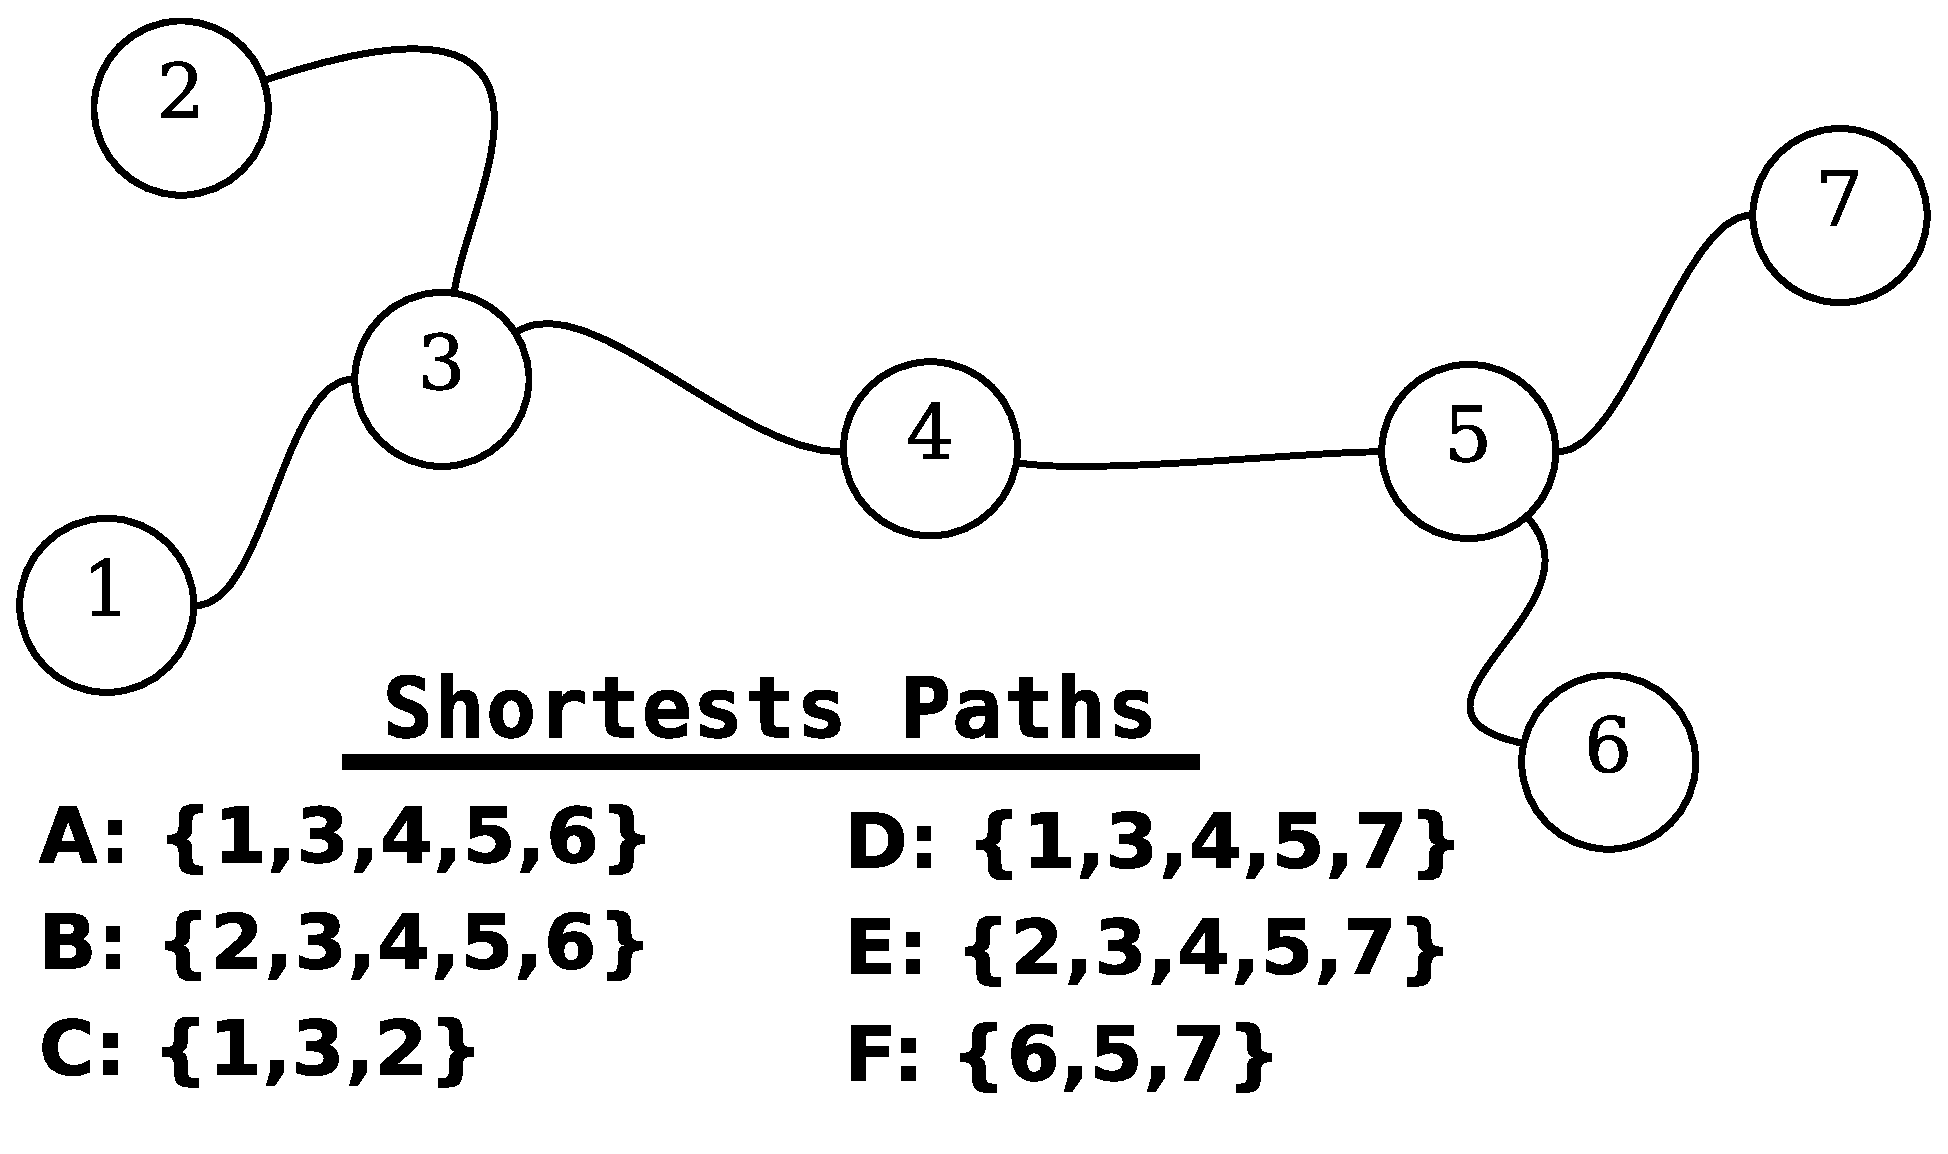
\includegraphics[width=0.5\textwidth]{figures/rxmap}
        \caption{Simple graph representation of a map.}
  \label{fig:rxmap}
\end{figure}


\subsection{Architecture}
We propose a system with a static \spath cache implemented in front of an existing \spath service (See fig. \ref{fig:routequery}) such that if the cache can answer a query then the result can be returned immediately. 

When the system receives a \spath query from a user (fig. \ref{fig:routequery}A) the system first checks if the cache (fig. \ref{fig:routequery}B) is able to answer the query. If the cache contains the query answer it is immediately returned (fig. \ref{fig:routequery}D), else the \spath algorithm is called (fig. \ref{fig:routequery}C) and the \spath result returned (fig. \ref{fig:routequery}D).

\begin{figure}
  \center
        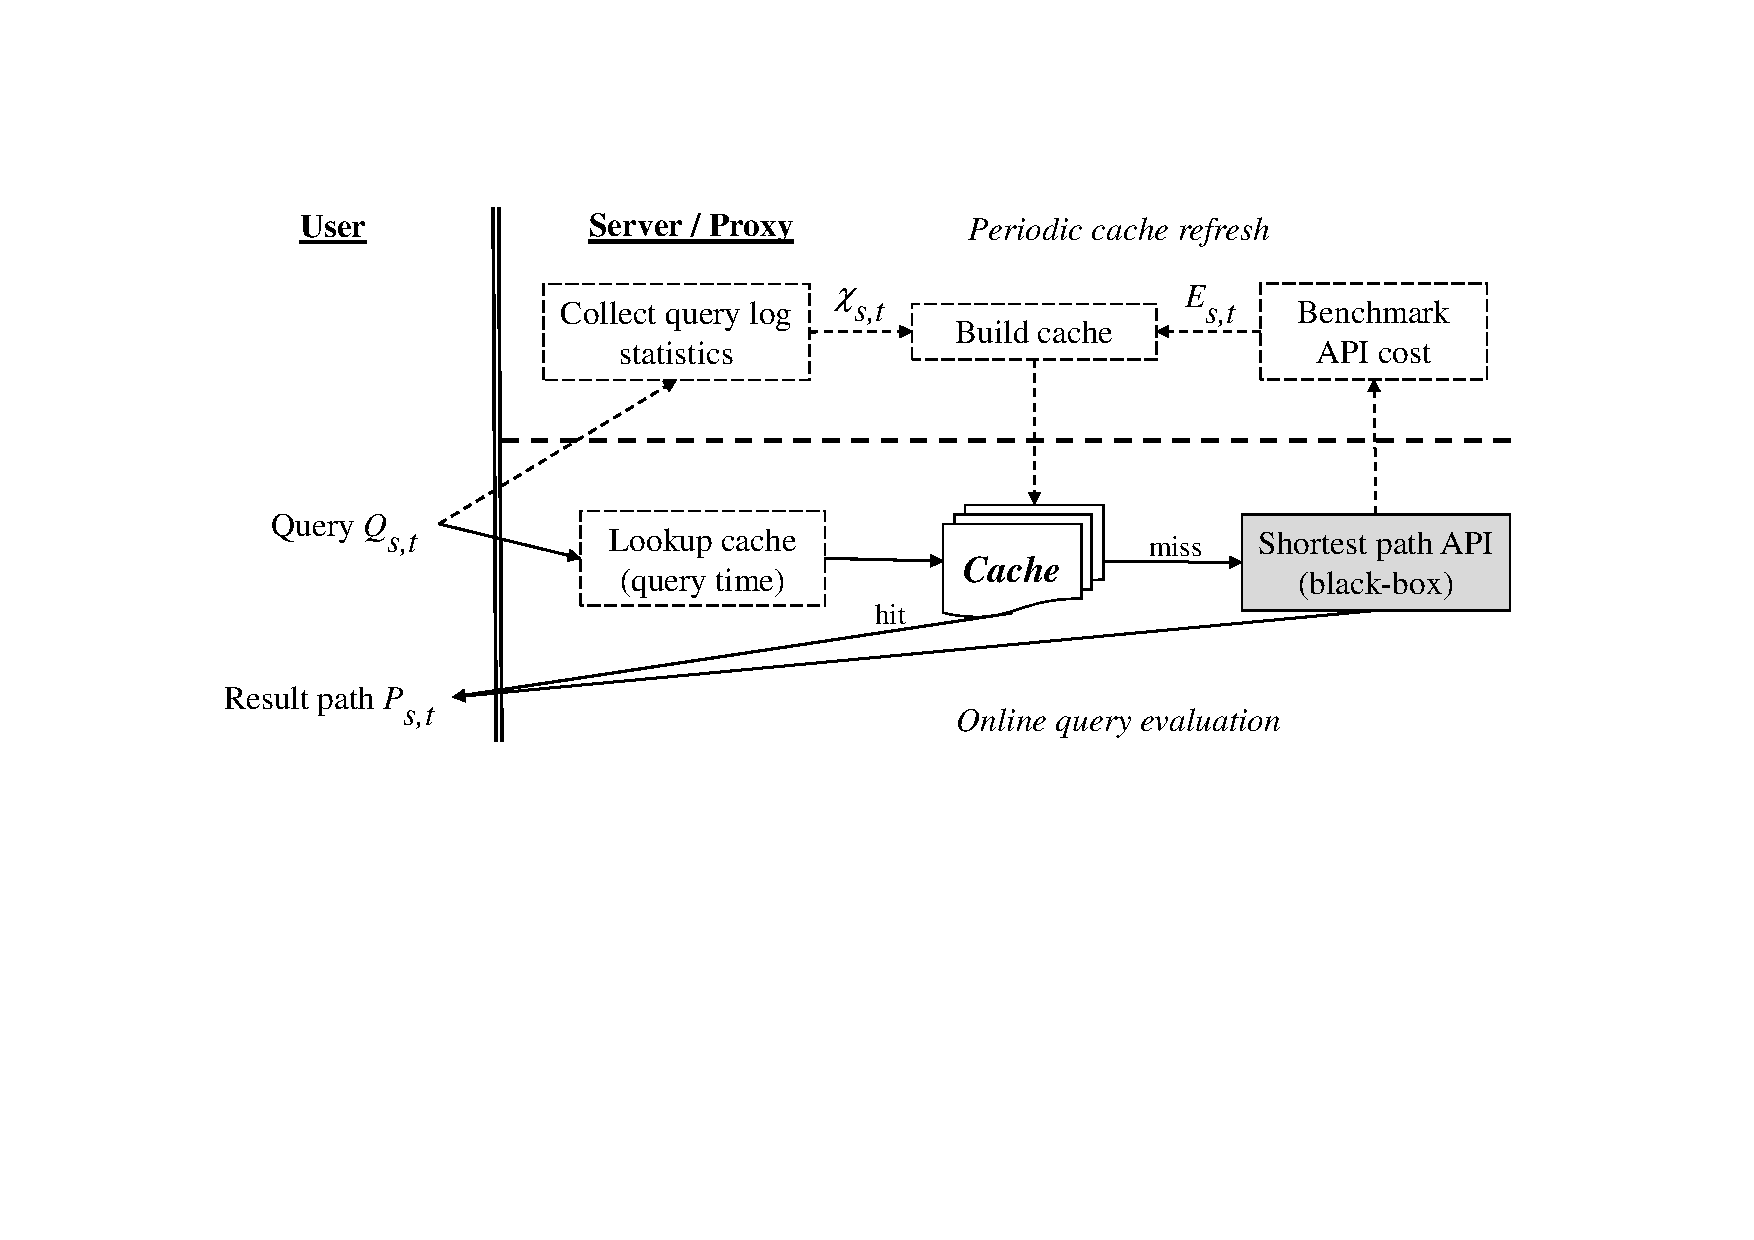
\includegraphics[width=0.5\textwidth]{figures/routequery}
        \caption{Buffer placement in \spath service providers system.}
  \label{fig:routequery}
\end{figure}


\subsection{Optimization Intend} \label{subsec:goals}

As the main problem with expensive \spath calculations is time needed, we use reduction in \textit{\cet} as the main optimization target and measurement to evaluate our success.
At a \spath service provider, the time spent to return a \spath result is essentially composed of two tasks: calculating the \spath and the overhead of query processing. 

We will address 3 subgoals:
\begin{enumerate}
\item \label{item:goal1}Reduce the gross \cet used to calculate \spathsns.
\item \label{item:goal2}Reduce the gross \cet spent on overhead in query processing.
\item \label{item:goal3}Determine the value of a sub-path in the cache.
\end{enumerate}

We want reduce the gross \cet of \spath calculations - goal 1 - as it is the most CPU intensive task at a \spath service, and therefor also the most time consuming. By using a cache we expect to see a negavite correlation between cache hit rate and \cet used on \spath calculation.

In a \spath service there will always be a some overhead associated with \spath query processing. Introducing a cache in front of the existing \spath service (fig. \ref{fig:routequery}B) will undeniably add more overhead as the cache needs to be queried for all queries submitted to the \spath service, regardless of whether it is able to answer the query or not. In order for the cache to be useful, the overhead introduced needs to be minimized (goal \ref{item:goal2}). We always have to make sure that the savings achieved by adding a cache to the system is greater than the overhead introduced.

The fact that the system will be using a static cache, and \spaths exhibit the \oss property, makes goal 3 - determining the value of a \spath subpath - very important. The ability to do goal \ref{item:goal3} well will have a direct influence on goal \ref{item:goal1} and  \ref{item:goal2}. If we fill the cache with useless \spaths we will end up calculating a \spath for all queries, as well as the overhead from checking the cache for each query. Solving goal 3 well is the most direct way to solve goal 1.

The \oss property states that every sub-path of a \spath is also a \spath. i.e \spath Q1 in table \ref{tab:queries} consists of: 
$\{Q_{1,3}, Q_{1,4}, Q_{1,5}, Q_{1,6}, Q_{3,4},$ $Q_{3,5}, Q_{3,6}, Q_{4,5}, Q_{4,6}, Q_{5,6}\}$, each one being a \spathns.

\begin{lemma}\label{lem:oss}
If a path $Q_{s,t}: v_s,v_{s+1},\ldots,v_t$ is a \spath, then $\forall$ $(v_k,v_l) | v_k \in Q_{s,t} \wedge v_l \in Q_{s,t}$ there is a  \spath $Q_{k,l}$ with start-/end-node in $v_k,v_l$, following a sub-path of $Q_{s,t}$ 
\end{lemma}

\begin{table}
\begin{tabular*}{\columnwidth}{|l||p{0.69\columnwidth}|}
\hline
\bf Abbreviation & \bf Meaning \\\hline
\spath          & Shortest Path \\\hline
$Q_{s,t}$	& \spathns: $\{v_s,v_{s+1},\ldots,v_t\}$ \\\hline
\acs{LRU}       & \acl{LRU} \\\hline
FIFO            & First In First Out \\\hline
\acs{SPS}       & \acl{SPS} \\\hline
\acs{CET}	& \acl{CET} \\\hline
\acs{OSS}	& \acl{OSS} \\\hline
\end{tabular*}
\caption{Table of Notation}
\label{tab:symbols}
\end{table}




% \subsection{helping text}
% \begin{enumerate}
% \item Introduce the problem setting in more detail than in the introduction and formally define the problem and what exactly we aim to solve in this paper.\\
% \item show where exactly the proposed cache is located in an online \spath service providers system.
% \item State goal 1(a) and 2(b)
% 	\begin{enumerate}
% 	\item Reduce the time spent executing the \spath algorithm. - The \spath algorithm is usually the single most CPU expensive task at a \spath service provider.
% 	\item Reduce the time spent on overhead. - Introducing a cache will also add some overhead, this overhead not desirable and should  be minimized.
% 	\end{enumerate}
% \item Introduce the overall setting which our solution work in and give a table of notation for reader reference.
% \end{enumerate}

%\section{Introduction} % Bookmark information

\subsection{Overview} % Bookmark information, displayed in the progress tree

\begin{frame}[red] %hmm.. thought i could change colour here :S
\frametitle{Goals}

Goal one
\begin{itemize}
\item Remove user identifying information from trajectories.
\end{itemize}

\vspace{3em}
Goal two, following Goal one\\

\begin{itemize}
\item Ensure enough information after removal of user information that:
	\begin{itemize}
	\item Similar sub-trajectories used to get from point A to B can be found
	\item Analysis of which roads are congested, and when; can be performed.
	\end{itemize} 
\end{itemize}
\end{frame}

\subsection{Related work}

\begin{frame}
\frametitle{Related work}

  \begin{itemize}
\item Protection of Identifiers on Trajectories

\item Trajectory classification
\end{itemize}

\end{frame}


\begin{frame}[red] %hmm.. thought i could change colour here :S
\frametitle{Protection of Identifiers on Trajectories}
Post processing of trajectories
	\begin{itemize}	 
	\item  Add information
		\begin{itemize}
			\item Add fake trajectories
		\end{itemize}
	\item Remove information 
		\begin{itemize}
			\item Remove sensitive segments of trajectories 
			\item collapse similar trajectories into one
		\end{itemize}
	\end{itemize}
\end{frame}


% \begin{frame}[red] %hmm.. thought i could change colour here :S
% \frametitle{Trajectory classification}
% 
%   \begin{itemize}
% 	\item Similarity of trajectories
% 	\item Outlier detection
% 	\item Congestion analysis
%   \end{itemize}
% \end{frame}

%\section{Privacy Profile}

\begin{frame}[red]
\frametitle{Privacy Profile}
\begin{itemize}
\item Settings
\item t-anonymity
\item PSR
\item Protection types and schemes
\end{itemize}
\end{frame}

\subsection{Settings} % Bookmark information, displayed in the progress tree

\begin{frame}[red] %hmm.. thought i could change colour here :S
\frametitle{Settings}

Users Can
\begin{itemize}
	\item Set both globally and locally
	\begin{itemize}
		\item Temporal sensitivity
		\item Spatial sensitivity
	\end{itemize}
	\item Define a PSR
	\item Have multiple profiles.
\end{itemize}

\vspace{1em}
\begin{definition}[Privacy Profile]
$\left(stime,etime,d_s, d_t,\{PSR \} \right)$
\end{definition}

\end{frame}



\subsection{PSR} % Bookmark information, displayed in the progress tree


\begin{frame}[red] %hmm.. thought i could change colour here :S
\frametitle{PSR}

\begin{definition}[PSR]
A PSR $p$ is a tuple $(p_{edges}, d_s, d_t, class)$ where $p_{edges}$ is the set of tuples $\{(e, e_{from}, e_{to} | 0 \leq e_{from} < e_{to} \leq e_{length})\}$ which is sensitive. 
$e \in \mathbf{E}$ and $e_{from}, e_{to}, e_{length} \in \mathbb{R}$. 
$e_{from}/e_{to}$ specifies on $e$ the start-/end-location covered by $p_{cover}$. If $e$ is fully included in $p_{cover}$, $e_{from}/e_{to}$ is equal to $0/p_{length}$.
$d_s, d_t, class \in \mathbb{N}$ is respectively the spatial sensitivity, the temporal sensitivity, and the PSR classification
\end{definition}

\end{frame}

\begin{frame}[red] %hmm.. thought i could change colour here :S
\frametitle{PSR Classes}

\begin{table}
%\begin{tabular*}{0.8\columnwidth}{|p{0.2\columnwidth}|l|p{0.25\columnwidth}|}
\begin{tabular}{|l|l|}
\hline
\bf Classification	& \bf Scheme \\\hline		
Public Service Point	& AS \\\hline
House			& ASTI,RS \\\hline
Route w. endpoints	& AS, ASTI, RS  \\\hline
Route w/o endpoints	& AS, ASTI, RS  \\\hline
\end{tabular}
\end{table}
\vspace{1em}

Protection Schemes
\begin{itemize}
	\item AS - Always Sensitive.
	\item ASTI - Always Sensitive within a time interval.
	\item RS - Rarely Sensitive.
\end{itemize}
\end{frame}


\subsection{Time Period}
\begin{frame}[red]
\frametitle{Time Period}
\begin{columns}
	\begin{column}{0.5\textwidth}
		\only<1>{ 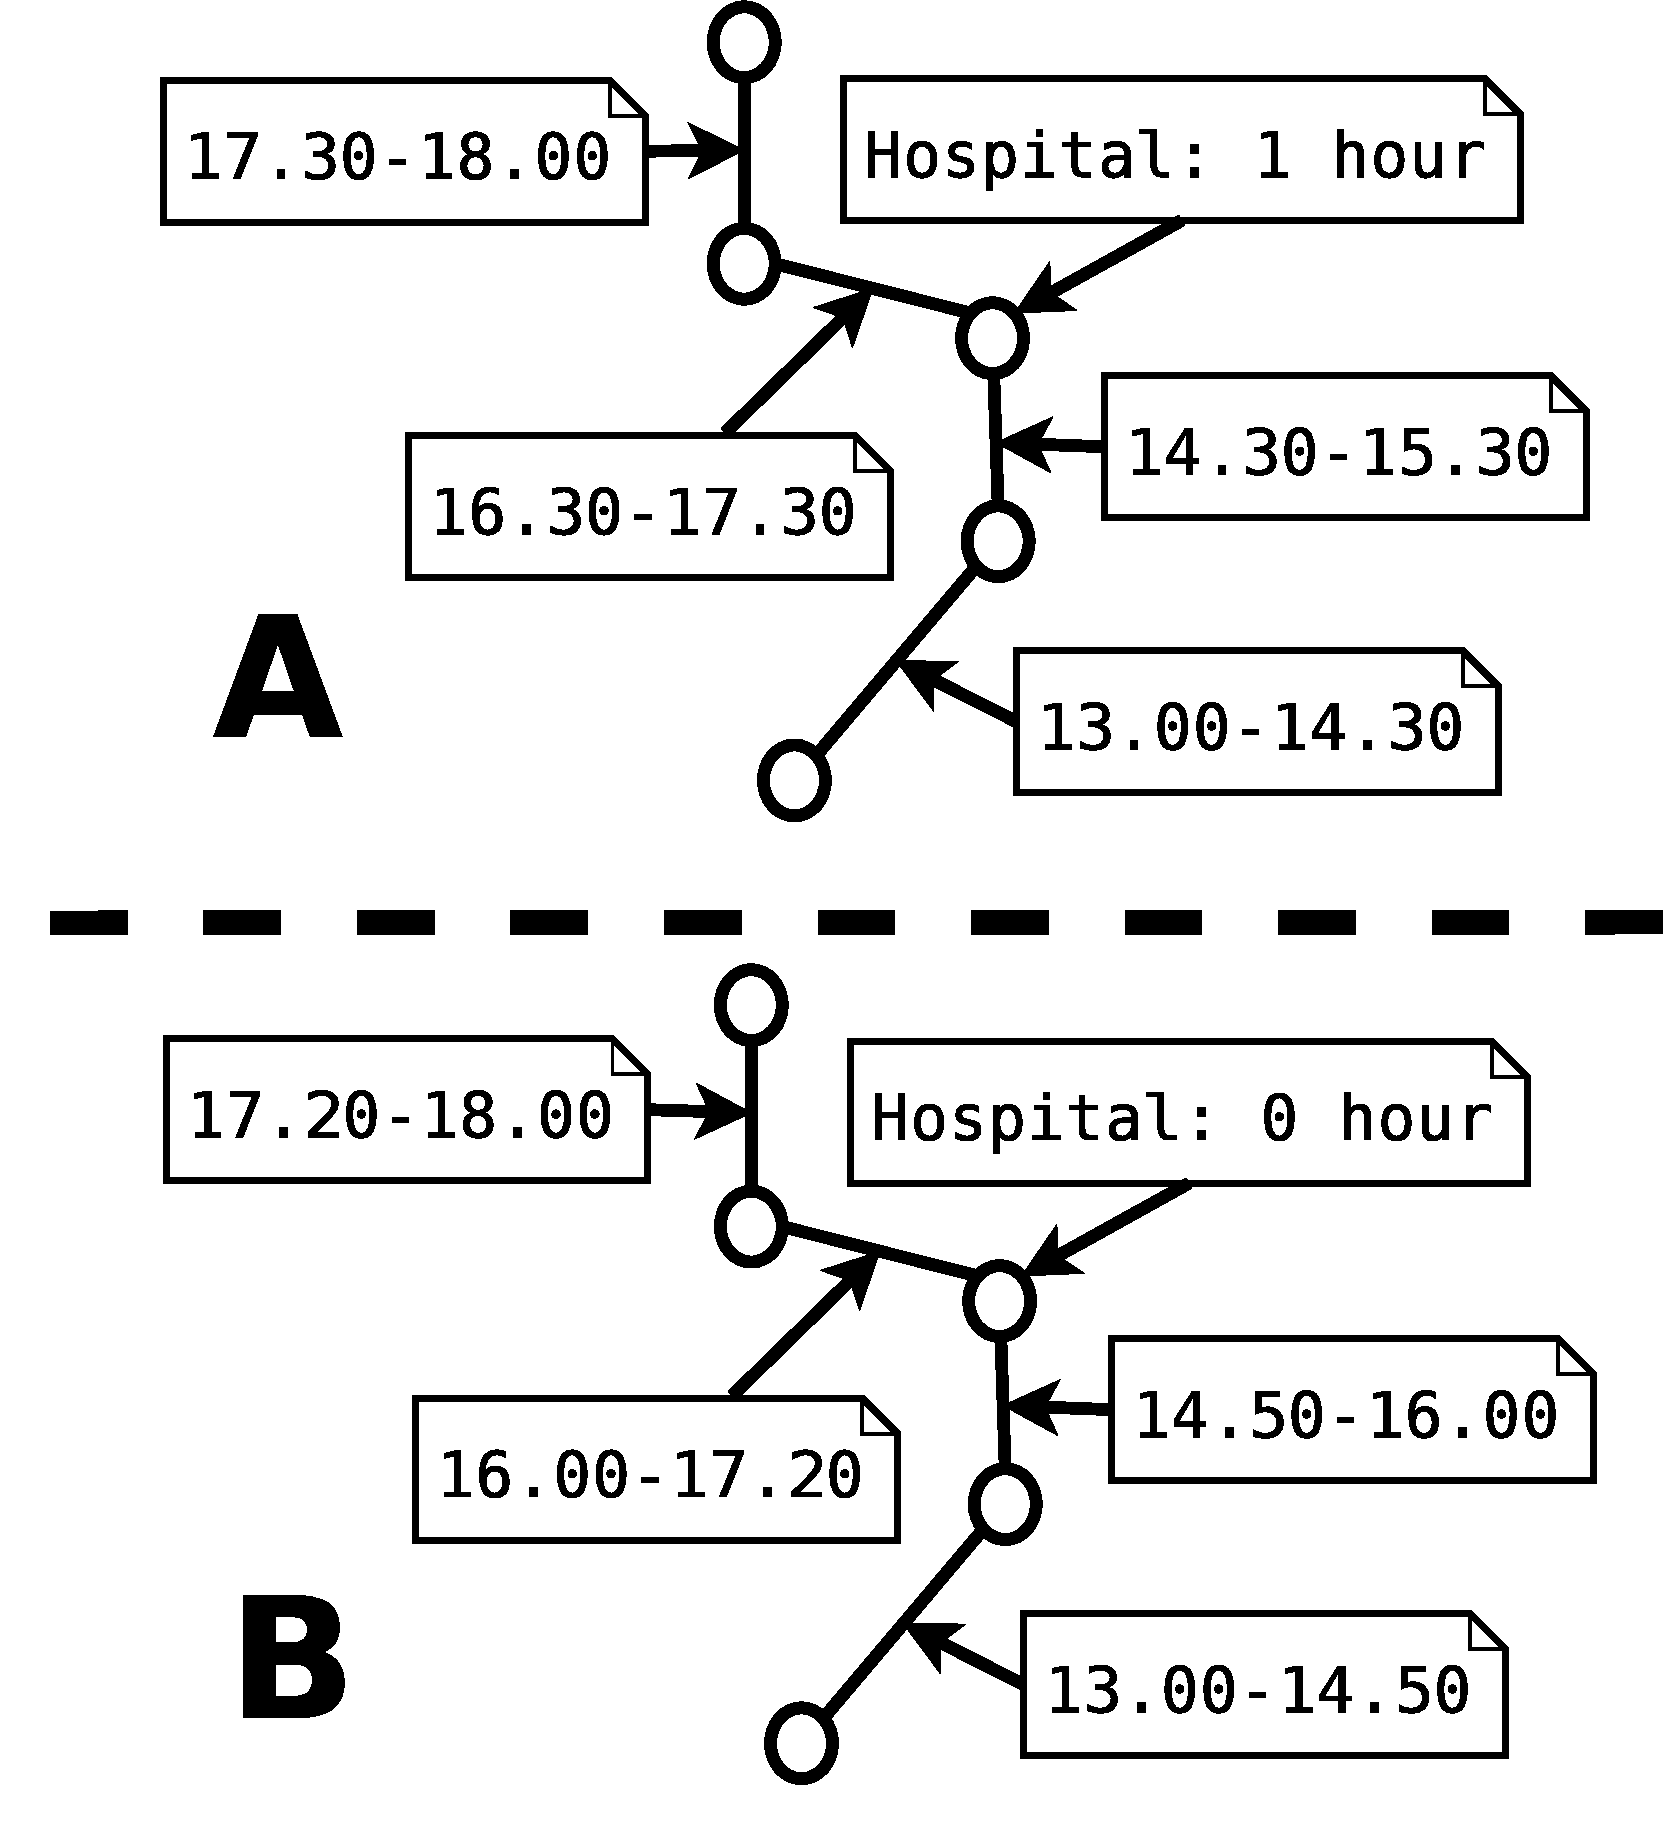
\includegraphics[scale=0.16]{images/trajecAdjustTime.pdf}}
	\end{column}
	\begin{column}{0.5\textwidth}
		\only<1>{ 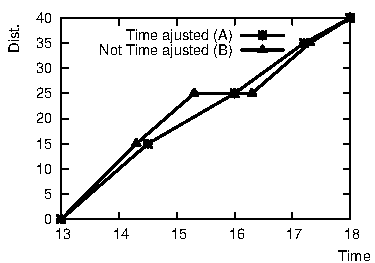
\includegraphics[scale=0.8]{images/trajecAdjustTimeGraph.pdf}}
	\end{column}
\end{columns}

\end{frame}

\subsection{t-anonymity} 
\begin{frame}[red] %hmm.. thought i could change colour here :S
\frametitle{t-anonymity}
\begin{definition}[t-anonymity]
Given $\mathbf{T}$, the set of trajectories and $p_{edges}$, the set of edges covering a sensitive part of trajectory $\gamma$. 

Let $\Gamma \subseteq \mathbf{T}$ be all trajectories which subtrajectories intersect with $p_{edges}$. $\Gamma' \subseteq \Gamma$ be all trajectories where, for edges intersecting with $p_{edges}$, at each timestamp of $\gamma$ their timestamps lie within a time period $TP$ symmetric around the timestamp of $\gamma$.

$\Gamma'$ is said to satisfy t-anonymity with respect to $TP$ and $\gamma$ iff $\Gamma'$ contains at least $t-1$ other trajectories.
\end{definition}
\end{frame}
%\section{Conclusion and Future Work}\label{sec:future}



summation of each goal from the problem setting for each goal argue we solved it well (recap key results and partial conclusions from applicable sections).






% In this paper we develop a novel Privacy Profile which enable users to easily specify their privacy requirements both spatially and temporally for trajectories.
% 
% To show the Privacy Profile usefull we develop framework with a high level of user privacy and providing a platform for service providers and traffic analysts to have high quality data to perform analysis and services on.
% 
% We have argued that the Privacy Profile provide: 
% {\it Usability} The user can specify his privacy requirements both spatially and temporally, and at more than one level. Is {\it Practical} The user does not need to interact with the client once a Privacy Profile is set up. The data input format is the same as the data output format making the anonymized data usable by existing approaches working on trajectory datasets allowing the user to choose from more existing services. It is {\it Flexible} Users can specify sensitivity at several levels and they can make several profiles which are active at different times or in contexts.
% 
% We have additionally introduced the system parameter $\mathbf{D}$ which guaranties a minimum level of data integrity, ensuring that analysis of the anonymized dataset can still be possible.
% 
% In the future it would be interresting to test the approach on real world trajectory dataset to measure performance and examine which values of $D$ might be appropriate to ensure a level of data quality usable by existing classification approaches for trajectories.
\end{document}

%General
%
%    * Is it clear where the paper was published and by whom?
%    * Does the talk have a concrete motivating example very early?
%    * Are unfamiliar abbreviations introduced and used appropriately?
%    * Is the main problem addressed in the paper clearly stated?
%    * Does the presentation have concrete and minimal examples of core ideas?
%    * Are dynamics, e.g., searching a tree presented using animation techniques?
%    * Are the listeners background use appropriately, e.g., no need to tell what an array is, however must tell what the XY++-Tree is?
%    * Is there a reasonable number of slides in total in the presentation?
%
%Figures
%
%    * Are complicated figures presented in sufficient details?
%    * Are the symbols used in the figures clear to the listeners?
%
%Performance Graphs
%
%    * Is data, queries, modification, and transactions appropriately introduced?
%    * Are the axis on performance graphs clearly explained?
%    * Are the main conclusion from the graph clearly stated?
%    * Is there only one graph per slide (or are graphs compared)?
%
%Critique
%
%    * Is the critique relevant and fair?
%    * Is the critique balanced?
%    * Is the critique points concrete, i.e., not "it is a good paper"?
